\documentclass[8pt,a5paper]{acm_proc_article-sp}
% fix umlauts
\usepackage[ngerman]{babel}
\usepackage[utf8]{inputenc} 
\usepackage[T1]{fontenc}  % Times new Roman
\usepackage{mathptmx}
\usepackage[]{blindtext}
\usepackage[a5paper, left=1.70cm, right=1.20cm, top=1.30cm, bottom=1.40cm]{geometry}
\usepackage{epstopdf}
% balance columns. original from acm doesn't work
\usepackage{balance}
% colors
\usepackage[compact]{titlesec}
\usepackage{natbib}
\titlespacing{\section}{0pt}{*0.7}{*0.5}

\usepackage[nolist]{acronym}
 
%\usepackage[usenames,dvipsnames]{xcolor}
\usepackage[greyscale]{xcolor} 
% automatic crosslinks
\usepackage[hyphens]{url}
\usepackage[colorlinks=false,
            allbordercolors={0 0 0},
            pdfborderstyle={/S/U/W 0.5}]{hyperref}
%glossaries
%\usepackage{makeidx}
%\makeindex
%\usepackage[nomain]{glossaries}
%\makeglossaries
%\makeindex

\newcommand{\glspl}[1]{{#1}}

% http://en.wikibooks.org/wiki/LaTeX/Glossary
% http://mirror.informatik.uni-mannheim.de/pub/mirrors/tex-archive/macros/latex/contrib/glossaries/glossariesbegin.pdf

% Definitionsliste
\newcommand{\defitem}[1]{\item[#1]\phantomsection\label{#1}\hfill\\} 
\newcommand{\defref}[1]{\hyperref[#1]{#1}} 
\newcommand{\rem}[1]{}
% Marking colors
\definecolor{todo}{rgb}{1,0.2,0.2}
\definecolor{reconsider}{rgb}{0.6,0.6,0.3}
\newcommand{\todo}[1]{{\color{todo} #1}}
\newcommand{\reconsider}[1]{{\color{reconsider} #1}}

% Hurenkinder und Schusterjungen verhindern
\clubpenalty10000
\widowpenalty10000
\displaywidowpenalty=10000


\graphicspath{{img/}{./}}
\usepackage{graphicx}
\title{Portable System to Detect driver drowsiness with Body Sensors (PoSDBoS) \titlenote{ \scriptsize 
  \flushleft Betreuer Hochschule:  \ \ Prof. Dr. Martinez\\ 
  \qquad \qquad \qquad \qquad \quad \ \  Hochschule Reutlingen\\ 
  \qquad \quad \quad \quad \qquad \qquad \ \ Natividad.Martinez@Reutlingen-\\
  \qquad \qquad \qquad \qquad \quad \ \ University.de \\
  
\includegraphics[width=1.8cm]{iot_hs_rt} \ \ \quad Master Project IoT 2016\\
  \ \ \\
  31. Juli 2016, Hochschule Reutlingen\\ 
  \copyright  ~ 2016 Paul Pasler}}


\numberofauthors{3}
\author{
	\alignauthor
	  \center
		\aufnt{Paul Pasler}\\
          \affaddr{Reutlingen University}\\
        \textbf{\textsf{Paul.Pasler@Student.Reutlingen-University.DE}}
}


\begin{document}
\begin{acronym}
\acro{FAS}{Fahrerassistenzsystem}
\acro{FASs}{Fahrerassistenzsysteme}
\acro{ME}{Müdigkeitserkennung}
\acro{MESs}{Müdigkeitserkennungssysteme}
\acro{ADAS}{Advanced Driver Assistance System}
\acro{ADASs}{Advanced Driver Assistance Systems}
\acro{bspw}{beispielsweise}
\acro{RTU}{Reutlingen University}
\acro{BS}{Körpersensoren}
\end{acronym}



\maketitle
\sloppypar{
\begin{abstract}
\acl{FASs} sind aus modernen Fahrzeugen nicht mehr wegzudenken. \acl{ME} hilft Sekundenschlaf oder müdigkeitsbedingte Unachtsamkeit zu vermeiden und verhindert somit schwere Unfälle. Systeme mit \acl{BS} zeigen in verschiedenen Studien sehr genau Ergebnisse und erkennen Müdigkeit frühzeitiger als andere Ansätze. In der vorgelegten Arbeit wurde ein solches System mit einem Elektroenzephalogramm (EEG) umgesetzt und getestet. Hierfür wurden Testdaten aufgenommen, verarbeitet und mit einem künstlichen Neuronalen Netz klassifiziert, sodass der aktuelle Status des Fahrers "`Wach"' oder "`Müde"' unterschieden werden konnte.
\end{abstract}

\keywords{
\acl{FAS}, \acl{ME}, Elektroenzephalogramm, Signalverarbeitung, Machine Learning, Neuronales Netz
}

\category{A.0}{ACM}{
Experimentation
}


\section{Einleitung}
\label{chap:intro}

\acl{FASs} sind innerhalb weniger Jahren von der Oberklasse in die Mittel- und Kleinwagenklasse vorgedrungen. Die Unternehmensberatung Strategy Analytics schätzt, dass in den nächsten Jahren sechs mal soviele \acl{FASs} verbaut werden als heute \cite{strategy_analytics}. Sie bieten dem Fahrer erhöhten Komfort (bspw. Tempomat) oder erhöhen die Sicherheit (bspw. Notbremsassistent). Laut der Boston Consulting Group, könnte der flächendeckende Einsatz von \acl{FASs} die Unfallrate um ein knappes Drittel zurückgehen lassen \cite{bcgperspectives}. 

\begin{figure}[h] 
  \begin{center}
    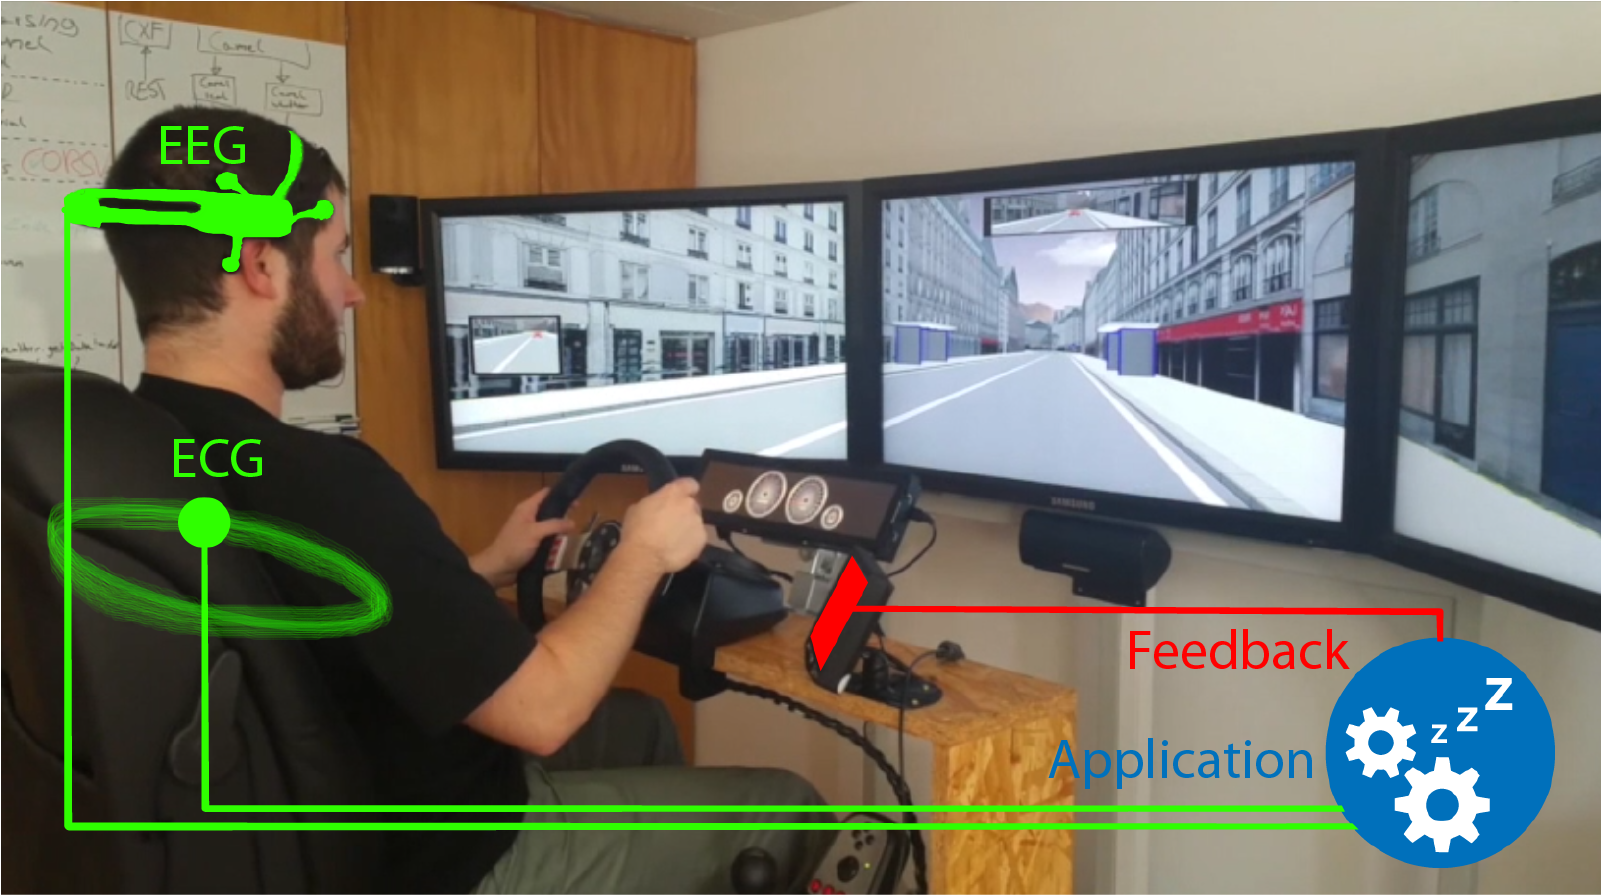
\includegraphics[width=\columnwidth]{aufbau}
    \caption[Skizze des Systemaufbaus]{Skizze des Systemaufbaus: \acl{BS} (Elektroenzephalografie / Elektrokardiogramm) liefert Daten an die Applikation und ein Feedback-Device warnt den müden Fahrer. Bild zeigt den Fahrsimulator der \acl{RTU}. \label{fig:sketch}}
  \end{center}
\end{figure}

Zu Gruppe der Sicherheitsrelevanten \acl{FASs} gehört auch die \acl{ME}. Beispielsweise rät die \acl{ME} "`Attention Assist"' von Daimler dem Fahrer, zu gegebenen Anlass, eine Pause einzulegen und zeigt ein Kaffeesymbol im Cockpit an \cite{Daimler}. So wird müdigkeitsbedingte Unachtsamkeit oder Sekundenschlaf, die oftmals die Folge von schweren Unfälle sind, entgegengewirkt.

In Deutschland wurden 2015 rund 2,5 Mio. Unfälle polizeilich aufgenommen, die Zahl der Verkehrstoten liegt bei 3.450 \cite{accident_statistic}. Neben überhöhter Geschwindigkeit, zählt laut dem Deutschen Verkehrssicherheitsrat Müdigkeit zu den häufigsten Unfallursachen und ist damit für jeden fünften schweren Unfall verantwortlich \cite{dvr_statistic}. Dies verdeutlicht das Potential einer frühzeitigen Erkennung von Müdigkeit und einer Meldung an den Fahrer.

\problemDetail

Daraus ergeben sich Anforderungen für ein multimodales System zur \acl{ME}  (Abb. \ref{fig:sketch}). Es existieren bereit diverse Systeme, denen es jedoch oftmals an Komfort und Portabilität mangelt. Ziel dieser Arbeit ist die Entwicklung einer solchen Anwendung mit einem EEG-Headset. 
Dessen Signale werden verarbeitet und mit einem KNN klassifiziert, um den Fahrer rechtzeitig vor Übermüdung und deren Folgen zu warnen.
Statt einem klassischen EEG, wie es in der Medizin eingesetzt wird, wird ein EPOC Emotiv genutzt, dadurch soll die Beeinträchtigung des Fahrers verringert werden. Auch wenn sich selbst dieser Ansatz weniger für den Serienbetrieb eignet, wird das Handling deutlich verbessert. So kann das gesamte System beispielsweise für die Validierung von berührungslosen Systemen (bspw. Kamerabasiert) verwendet werden. Das ganze System soll leicht portierbar sein, um es in einem echten Fahrzeug testen zu können. Jedoch werden die notwendigen Testdaten im Rahmen des Projekts im Fahrsimulator der \acl{RTU} aufgenommen.

\tofc


\section{EEG Headset}
\label{chap:eeg}
Für das Projekt wurde ein EMOTIV Epoc+ EEG Headset \footnote{\url{http://emotiv.com/epoc}} (Abb \ref{fig:epoc_eeg}) verwendet. Es besitzt 14 EEG Kanäle, sowie ein Gyroskop und sendet seine Daten via Bluetooth an den Rechner. Das Headset wird über den Kopf gestülpt und besitzen an den Sensorenden einen Filz der mit Kochsalzlösung befeuchtet wird. 

\begin{figure}[h] 
  \begin{center}
    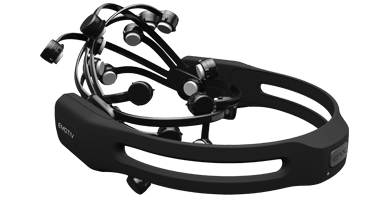
\includegraphics[width=0.75\columnwidth]{epoc_eeg}
    \caption[EMOTIV Epoc]{Das EMOTIV Epoc+ EEG Headset wird einfach über den Kopf gestülpt.\label{fig:epoc_eeg}}
  \end{center}
\end{figure}

Die Sensoren Anordnung ist an das internationale 10-20 System \cite{10-20}  angelehnt (\ref{fig:epoc_sensors}). Hierbei handelt es sich um eine standardisierte relative Anordnung der Elektroden. Die Rohdaten werden Abtastrate von 128 geliefert und enthalten neben dem Wert auch die Signalstärke (Qualität). Leider liefert die mitgelieferte SDK die Rohdaten nicht in Echtzeit, weshalb die Open-Source Lösung Emokit\footnote{\url{https://github.com/openyou/emokit}} eingebunden wurde.

\begin{figure}[h] 
  \begin{center}
    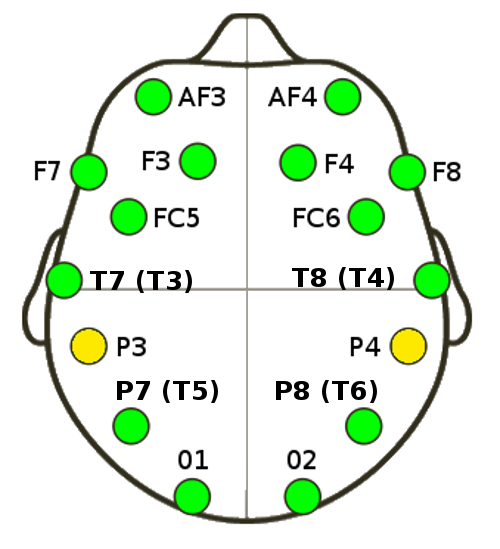
\includegraphics[width=0.5\columnwidth]{epoc_sensors}
    \caption[EEG Sensoren]{Die 14 Kanäle (Grün), sowie die beiden Qualitätssensoren (Gelb).\label{fig:epoc_sensors}}
  \end{center}
\end{figure}

\section{Stand der Technik}
\label{chap:state}
Systeme zur Erkennung von Müdigkeit versuchen mit verschiedenen Parametern herauszufinden, ob sich die Person (der Fahrer) noch in einem aufmerksamen Zustand befindet. Die lässt sich in drei Bereiche unterteilen: Fahrverhalten, Computer-Vision (CV) und Körpersensoren. 
\comp

Ansätze mit einem EKG allein, zeigten in verschiedenen Arbeiten kein eindeutiges Ergebnis \cite{Vicente_6164509}\cite{Rogado_4913155}. Beide versuchten Informationen aus der Herzfrequenzvariabilität zu erhalten und diese zu klassifizieren. 
Khushaba et al. \cite{Khushaba_5580017} versuchten EEG, EKG und EOG zu verbinden und verglichen verschiedene Kombinationen. Mit einem "`fuzzy wavlet"' basierten Algorithmus wurden die Signale aufbereitet und zeigten, dass ein EEG alleine bereits ausreicht. Die Kombination eines EEG mit EKG bzw. EOG verbesserte das Ergebnis nicht signifikant. Auch Johnson et. al \cite{Johnson11} kamen zu der Erkenntnis, dass ein EEG ausreicht und das eingesetzte EOG nicht benötigt wird. Subasi \cite{Subasi:2005:ARA:1707423.1707550} konnte mit einem EEG die Zustände "`Wach"', "`Schläfrig"' und "`Schlafend"' unterscheiden. Die Wavelet-Transformation und das genutzte künstliche Neuronale Netz (KNN) führten zu einer Erkennungsrate von 93\%. Vuckovic et al. \cite{Vuckovic2002349} fanden den besten Algorithmus für die Initialisierung des KNNs: Der Learning Vector Quantization Algorithmus. Im Vergleich mit EEG-Experten erreichte das KNN eine Übereinstimmung von 90\%. Huang et al. \cite{Huang_548971} nutzten ein Hidden Markov Modell zur Erkennung und erreichten eine gute Erfolgsrate. Lin et al. \cite{Lin05eeg-baseddrowsiness} nutzten die Unabhängige Komponenten Analyse (UKA) und Lineare Regression (LR) und konnten zeigen, dass hiermit  bis zu 88\% richtige Ergebnisse erzielt werden können. 

Die betrachteten Arbeiten unterstreichen die Eignung von Körpersensoren  um Müdigkeit zu erkennen. Die Stärken im Bereich Präzision und Korrektheit, im Vergleich zu Verhaltensanalyse oder CV-Techniken, zeigten sich in der Erkennungsrate. Den Komfort betreffend bleiben Körpersensoren jedoch hinter den anderen Ansätzen zurück. 

Verhaltensanalyse oder CV-Technik werden für die Arbeit nicht berücksichtigt und treten nur bei der Analyse / Markierung der Testdaten in Erscheinung. Gähnen, häufiges Blinzeln oder Abkommen von der Fahrspur, können Hinweise auf Müdigkeit sein. Treten diese Anzeichen auf, können die entsprechenden EEG-Sequenzen gelabelt werden können. 
Aufgrund seiner höheren Genauigkeit, gegenüber EKG oder EOG, wird für die Anwendung ein EEG genutzt. Ein multimodales System ist vorbereitet, aber nicht umgesetzt. Die betrachteten Arbeiten zeigen in verschiedensten Ausführungen sehr gute Ergebnisse (\textasciitilde 90\% \cite{Lin05eeg-baseddrowsiness}, \cite{Subasi:2005:ARA:1707423.1707550}), sodass es sich beim EEG um eine aussichtsreiche Grundlage handelt. 
Für die Klassifizierung nutzen die meisten Ansätze ein Künstliches Neuronales Netz  (KNN)\cite{Subasi:2005:ARA:1707423.1707550}\cite{Vuckovic2002349}\cite{wilson_890161}\cite{khalifa_893852}. Weitere Ansätze nutzen die Lineare Diskriminanten Analyse\cite{Vicente_6164509}\cite{Khushaba_5580017} oder ein SVM\cite{Park:2009:DDD:1667780.1667798}\cite{zhang_6513058}. Aufgrund der Häufigkeit in den anderen Arbeiten und der guten Bibliotheksunterstützung (PyBrain) wurde der Ansatz mit einem KNN weiter verfolgt. Die vorgestellten Lösungen arbeiten mit medizinischen oder selbst gebauten EEGs. Alle Ansätze wurden in einer simulierten Umgebung entwickelt und nie unter realen Bedingungen getestet. Aus der Analyse der verwandten Forschungsarbeiten ergeben sich Anforderungen an eine Anwendung zur \acl{ME}. 


\section{Testdatenbeschaffung}
\label{chap:data}
Um Daten von übermüdeten Fahrern zu erhalten, kann natürlich kein Versuch im Straßenverkehr durchgeführt werden. Die Fremd- und Eigengefährdung ist zu groß. Darum finden die Versuche in der Simulationsumgebung der \acl{RTU} statt. Für das Experiment wird im Fahrsimulator eine Nacht-Autobahnfahrt simuliert. Verschiedene Studien \cite{Engstrom_2322937}, \cite{Horne_1757738} legen nahe, dass sich Simulationen zwar von der Realität unterscheiden, dass  die Ergebnisse jedoch trotzdem valide und brauchbar sind.

Für den Versuch werden neben den rohen EEG Signalen, auch die Fahrzeugdaten, sowie ein Video der Simulation und des Fahrers aufgenommen. Weiterhin kann der Versuchsleiter Besonderheiten protokollieren (Abb. \ref{fig:experiment}).

\begin{figure}[h] 
  \begin{center}
    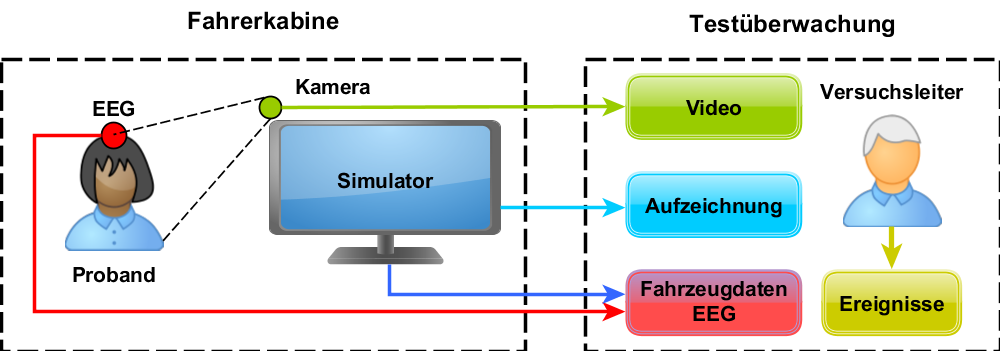
\includegraphics[width=\columnwidth]{experiment}
    \caption[Versuchsaufbau Experiment]{Der Versuchsaufbau für die Erkennung von Müdigkeit mit den Datenströmen aus der Fahrerkabine zur Testüberwachung. \label{fig:experiment}}
  \end{center}
\end{figure}

Im Versuch sollte der Fahrer, mit fortschreiten des Versuchs, immer mehr eindeutige Anzeichen von Müdigkeit zeigen. Dies kann durch verschiedene Versuchsparameter begünstigt werden. So zeigt eine Studie, dass Unfälle meist zwischen 2:00 - 6:00, sowie 14:00 - 16:00 Uhr passieren \cite{Horne_1757738}. Auch die Schlafmenge von weniger als 6 Stunden in der Nacht vor dem Experiment erhöht die Chance auf Anzeichen \cite{Engstrom_2322937}. Das Geschlecht oder Alter der Probanden ist nicht relevant. Vor dem Experiment sollten jedoch keine Drogen, Alkohol oder Kaffee eingenommen werden. Ein Führerschein ist von Vorteil, aber nicht zwingend notwendig.

Auch die Teststrecke (Abb. \ref{fig:drivingtask}) trägt zur Erhöhung der Müdigkeit bei. Monotone Autobahnfahrten die größtenteils geradeaus verlaufen, ohne andere Verkehrsteilnehmer und konstanter Geschwindigkeit führen eher zu einer Ermüdung. Nach diesen Kriterien wurde eine endlose zweispurige Autobahnkarte mit einer Geschwindigkeit von konstant 130Kmh erstellt. Sie spielt zudem Nachts und ist somit dunkel gehalten, was besonders anstrengend für die Augen ist. Die Simulation ist auf Bildschirm vermutlich noch anstrengender als eine echte Aussicht durch ein Autofenster.

\begin{figure}[h] 
  \begin{center}
    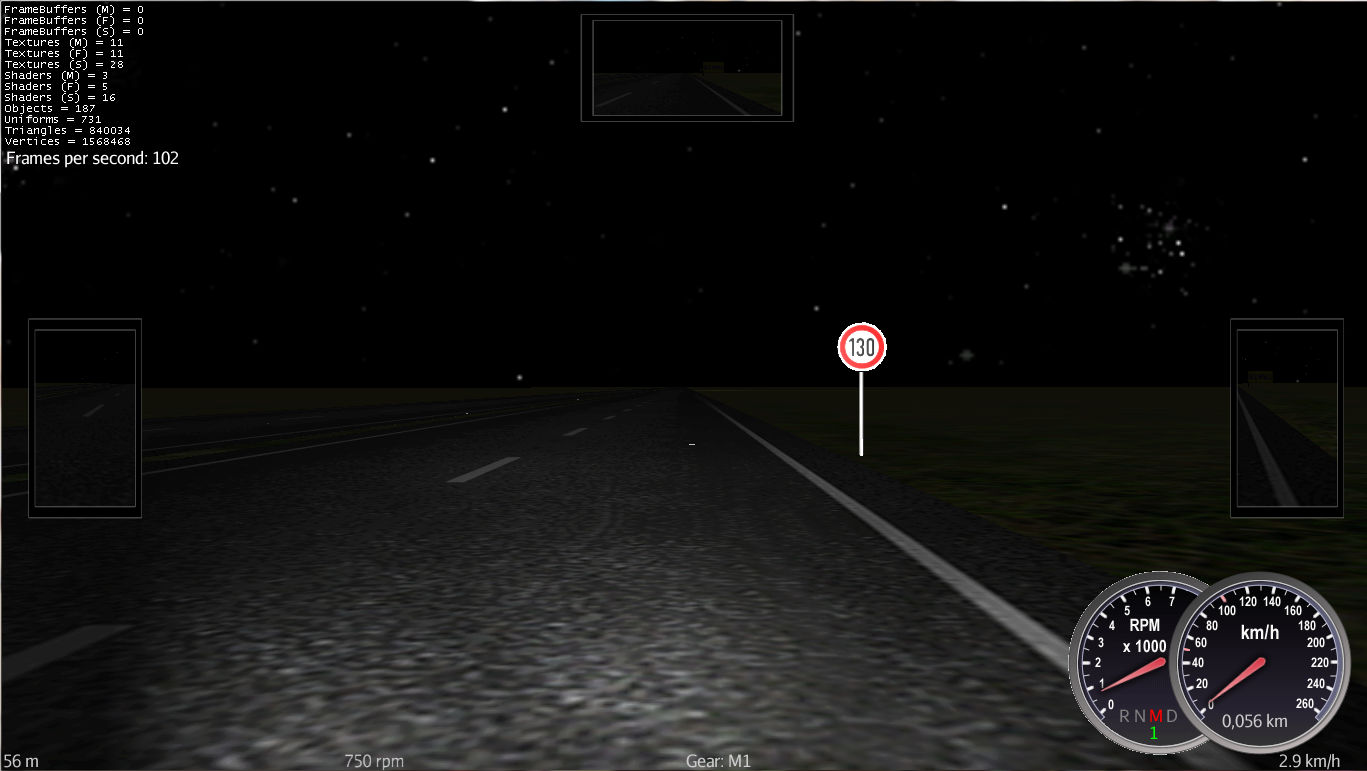
\includegraphics[width=0.75\columnwidth]{drivingtask}
    \caption[Driving Task Screenshot]{Die Autobahnkarte für den Versuch verläuft endlos geradeaus und spielt nachts bei konstanter Geschwindigkeit. \label{fig:drivingtask}}
  \end{center}
\end{figure}

Für einen Versuch werden 40 Minuten angesetzt. Fünf Minuten werden für eine kurze Einführung und Einrichten des EEGs, 30 Minuten für die Testfahrt und wieder fünf Minuten für eine kurze Selbsteinschätzung mit Fragebogen.

Anhand der aufgenommenen Daten werden nun Stellen gesucht, an denen die Testperson eindeutige Anzeichen von Müdigkeit zeigt. Eindeutig sind Verhaltensweisen wie häufiges Gähnen und Einnicken (Kopf fällt nach vorn) - diese Merkmale werden häufig in CV-Ansätzen genutzt. 
Auch Verhaltensmerkmale wie, von der Spur abkommen und heftig Gegenlenken oder deutliche Veränderungen der Geschwindigkeit können Anzeichen für eine Unachtsamkeit aufgrund von Müdigkeit sein. Diese Stellen werden dann in den EEG Daten mit dem Label "`Müde"' markiert, alle anderen mit "`Wach"'. Die EEG Sequenzen können dann auf eindeutige Varianzen untersucht werden. 

Das Experiment wurde mit 4 Personen (m / w) durchgeführt. Das Einrichten des EEG-Headsets (alle Sensoren auf hoher Qualität) war aufwändiger als erwartet, klappte jedoch bei allen Personen. Aus organisatorischen Gründen, fand nur ein Teil der Experimente nachmittags statt, der Rest fuhr morgens. Die Teilnehmer hatte im Vorfeld verschieden lang geschlafen und bewerteten auch die jeweilige Schlafqualität unterschiedlich. Die Testpersonen gaben an, vor dem Experiment eher wach als müde zu sein. Alle Fahrer gaben an, schon einmal übermüdet gefahren zu sein, waren sich aber nicht einig, ob sie sich eine Müdigkeitserkennung in einen Neuwagen bestellen würden.

Nach der Testfahrt gaben alle Teilnehmer an, müder als vorher gewesen zu sein. Dies zeigt sich auch an visuellen Merkmalen in den letzten Minuten der Testfahrt. Wobei die Ausprägungen der einzelnen Fahrer durchaus unterschiedlich war. Visuelle Anzeichen von Müdigkeit waren den Testpersonen bekannt (Gähnen, häufige Positionswechsel, häufiges Blinzeln, trockene Augen) und konnten diese an sich selbst beobachten. Auch die Fahrweise zeigte teilweise deutliche Anzeichen von Unkonzentriertheit (Abkommen von der Spur, Schlangenlinien, zu niedrige / hohe Geschwindigkeit).

Die Eigen- und Außenwahrnehmung bestätigt die Hypothese, dass es während des Experiments zu einem Abfall der Wachheit kommt und sich dies an Hand der erwarteten Merkmale zeigte. Die Veränderungen der Aufmerksamkeit muss nun im EEG Signal extrahiert werden.


\section{Müdigkeitserkennung mit einem EEG-Headset}
\label{chap:implementation}

Abbildung \ref{fig:data_stream} zeigt die Gesamtübersicht des entwickelten Systems. 
\begin{figure*} 
  \begin{center}
    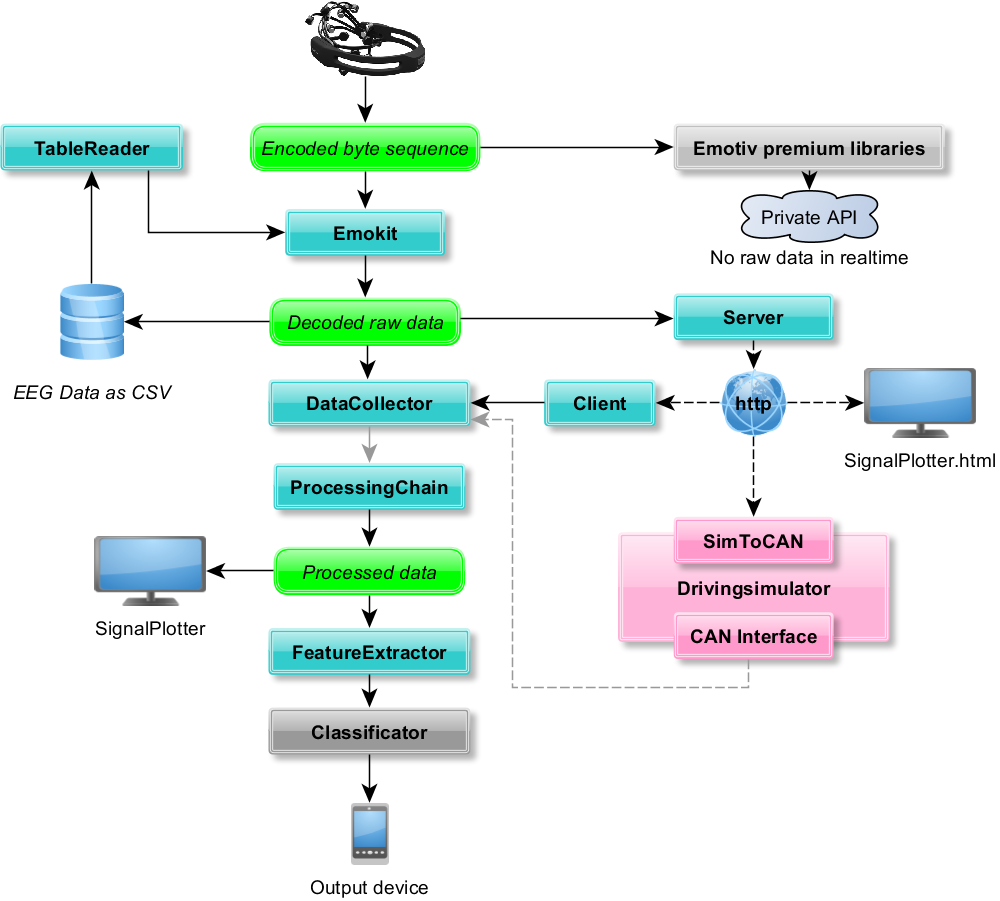
\includegraphics[width=\columnwidth]{data_stream}
    \caption[Aufbau der Anwendung]{Der Aufbau des entwickelten System zur Müdigkeitserkennung. Grün: Datenströme, Blau: Python Klassen der Anwendung, Gelb: bedingte Abzweigungen, Rosa: Klassen der Fahrsimulatorumgebung\label{fig:data_stream}}
  \end{center}
\end{figure*}
Alle blauen Klassen der Anwendung wurden in Python 2.7 implementiert. Der Fahrsimulator und seine Schnittstellen (rosa) in Java und C\#, die einzelnen Datenströme sind Grün gekennzeichnet. Bedingte Abzweigungen für alternative Wege in Gelb. Die Anwendung läuft verteilt auf dem DataCollector und dem Embedded PC. Die Datenquelle befindet sich auf dem DataCollector, von dort werden die Daten via CAN-Bus an den Embedded PC übertragen und verarbeitet (Abb. \ref{fig:data_stream_mapping}). 
\begin{figure}[h] 
  \begin{center}
    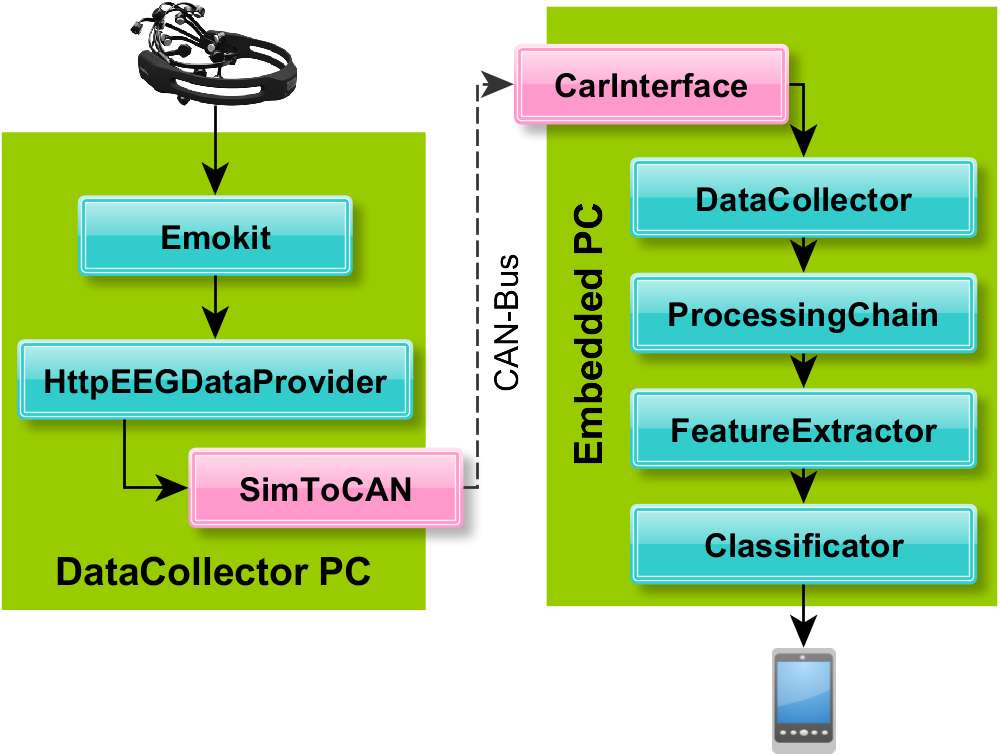
\includegraphics[width=\columnwidth]{data_stream_mapping}
    \caption[Einbettung der Anwendung]{Datenquelle und Verarbeitung sind verteilt im Fahrsimulator eingebettet. Die Übertrageung erfolgt via CAN-Bus. \label{fig:data_stream_mapping}}
  \end{center}
\end{figure}

\threadingSequence

Abschnitt \ref{sec:fetching} befasst sich mit den Rohdaten und deren Weiterreichung im System. Die Verarbeitung der Rohdaten ist Thema von Abschnitt \ref{sec:processing}. Im folgenden Abschnitt werden daraus die passenden Merkmale extrahiert. In Abschnitt \ref{sec:classification} wird die Arbeitsweise des Klassifikators näher beleuchtet. 




\subsection{Datensammlung}
\label{sec:fetching}
 
Das EEG Headset schickt enkodierte Byte-Sequenzen via Bluetooth, an die proprietären Emotiv Premium Libraries oder die Open-Source Lösung Emotkit (vgl. \ref{chap:eeg}). Die Emokit Klasse wurde für das Projekt leicht modifiziert, sodass sie sich ins System einfügt. So wurde Unterstützung für das neueste EPOC+ Modelle implementiert, sowie die Möglichkeit, gespeicherte Testdaten aus dem TableReader zu versenden (Demo-Modus ohne Headset). 
Die dekodierten Rohdaten enthalten 14 EEG Kanäle mit Wert und Qualität, die Gyroskopwerte in X- und Y-Richtung und einen Zeitstempel (Abb. \ref{fig:data_processing}). Mit einer Abtastrate von 128Hz sind das 128 * 16 = 2048 Werte pro Sekunde. Diese Daten können als CSV gespeichert werden, sowie an einen HTTP-Server oder direkt an den DataCollector übergeben werden. Über den Server integriert die SimToCAN Anwendung via HTTP die EEG Daten in den Fahrsimulator und das virtuelle Steuergerät.

\begin{figure}[h] 
  \begin{center}
    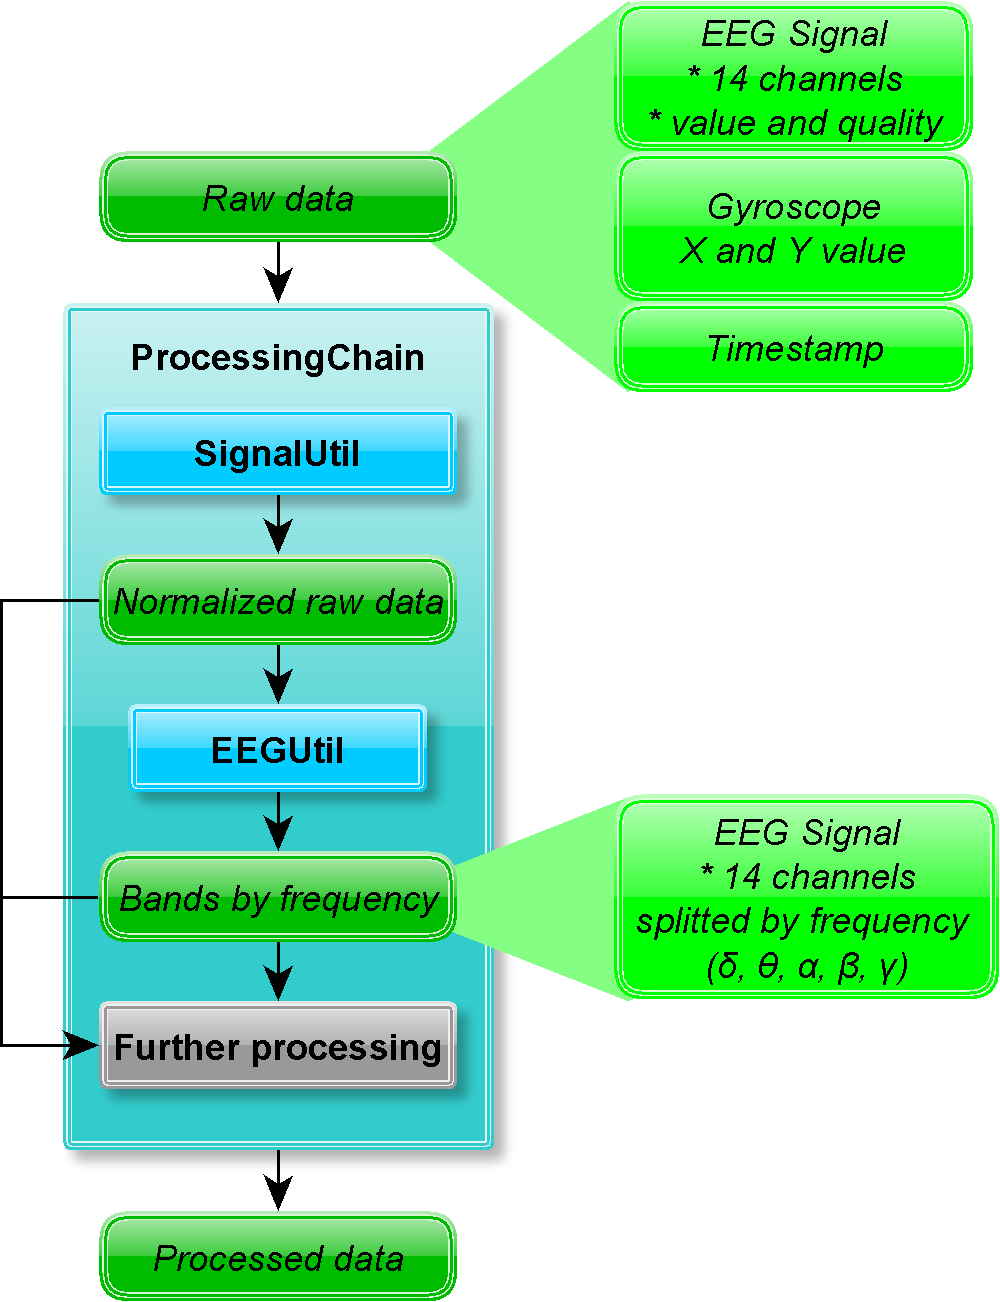
\includegraphics[width=\columnwidth]{data_processing}
    \caption[Datenverarbeitungskette]{Die Daten werden verarbeitet und dabei immer weiter reduziert. \label{fig:data_processing}}
  \end{center}
\end{figure}

Der DataCollector kann Daten direkt oder aus einem HTTP-Client empfangen. Die Schnittstelle zum CAR-Interface ist vorbereitet. So ist es möglich die Datensammlung und die Datenverarbeitung auf verschiedenen Rechnern durchzuführen.

Die Aufgabe der DataCollector-Klasse ist es, die einzelnen Signale in Sequenzfenstern von 128 Signalwerten zu aggregieren. Das ist die Abtastrate des EEG-Headsets und entspricht somit in etwa den Signalen einer Sekunde. Es sind zwei dieser Fenster implementiert und sie überschneiden sich in der Hälfte. So ist gewährleistet, dass signifikante Stellen nicht verloren gehen. Die Fensterfunktion ist ein simples Rechteck, sodass alle Werte gleich gewichtet werden. Eine andere Fensterfunktion bspw. mit Glockenkurvenerlauf (Hamming- oder Hann-Fenster) wäre einfach einzubauen. Auf den ersten Blick ist die Fensterlösung eine Verdopplung der Daten, jedoch fügt der DataCollector nur konfigurierte Kanäle hinzu, sodass sich die Datenmenge wieder deutlich reduzieren lässt. Im folgenden Abschnitt werden die gefilterten Sequenzfenster nun verarbeitet und aufbereitet.


\subsection{Datenverarbeitung}
\label{sec:processing}
Die gefilterten EEG-Sequenzen durchlaufen nun eine Verarbeitungskette (Abb. \ref{fig:data_processing}). 

Im ersten Schritt werden die Signale auf das Intervall 1 bis -1 normalisiert , dazu werden die Signale durch den jeweiligen Maximalwert bzw. Betrag des Minimalwertes geteilt. Dieses Vorgehen stellt sicher, dass die absolute Amplitude keinen Einfluss auf die Gewichtung im Klassifikator hat. Zudem wird die Datenmenge wiederum reduziert.

Im zweiten Schritt werden die Signale in Frequenzbänder (EEG-Bänder)  unterteilt. Hierzu werden bestimmte Frequenzbereiche aus dem Signal entfernt, sodass nur die gewünschten Frequenzen erhalten bleiben. Diese EEG-Bänder gliedern sich in folgende Frequenzbereiche und werden nach griechischen Buchstaben benannt:
\begin{itemize}
 \item $\delta$ : 0,1 bis < 4Hz
 \item $\theta$ :   4 bis < 8Hz
 \item $\alpha$ :   8 bis < 13Hz
 \item $\beta$  :  13 bis < 30Hz
 \item $\gamma$ :  > 30Hz
\end{itemize}
Den Frequenzbändern werden verschiedene Eigenschaften zugesprochen\\

\textbf{TODO Frequenzbänder}\\

Um die einzelnen Frequenzbänder zu erhalten ist eine Filterfunktion notwendig. Für die Anwendung wurde hierfür ein Buttworth-Filter\cite{Butterworth30} eingesetzt. Gleichung \ref{eq:butterworth} zeigt die Übertragungsfunktion mit $A_0$: Gleichspannungsverstärkung, $\Omega = \frac{f}{f_g}$: auf Grundfrequenz normierte Frequenz und $n$: Ordnung des Filters. Abbildung \ref{fig:butterworth_filter} zeigt exemplarisch Filterfunktionen verschiedener Ordnung mit den Grenzen von 500 bis 1250Hz. Alle Frequenzen darunter und darüber werden deutlich abgeschwächt bzw. gehen gegen null. Der Butterworth-Filter verläuft nahe Eins im gewünschten Bereich, fällt an den Grenzen ab und stellt sicher, dass das Signal an den Grenzen um $\frac{1}{\sqrt{2}} \approx 0.7071$ gemindert wird. Je höher die Ordnung, desto steiler geht die Funktion durch die angegebenen Grenzen. Der Filter lässt sich gut in Hardware realisieren.

\begin{equation} \label{eq:butterworth}
\left|\underline{A}\right|^2 = \frac{A_0^2}{1+ k_{2n} \Omega ^{2n}}
\end{equation}

\begin{figure}[h] 
  \begin{center}
    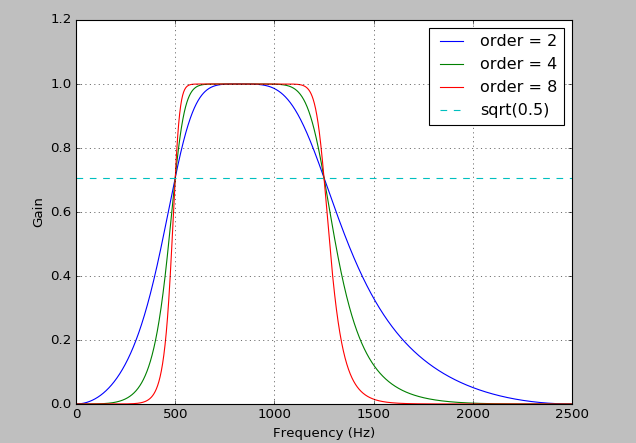
\includegraphics[width=5.5cm]{butterworth_filter}
    \caption[Butterworth-Filter]{Die Filterfunktion eines Butterworthfilters 2., 4,. und 8. Ordnung im Frequenzbereich von 500 bis 1250Hz. \label{fig:butterworth_filter}}
  \end{center}
\end{figure}

\subsection{Mermalsextraktion}
\label{sec:extraction}
Nach der Aufbereitung und Verarbeitung der EEG-Signale, müssen nun signifikante Daten extrahiert und eine Merkmalsmenge erstellt werden, welche vom Klassifikator erkannt werden kann. 

Aus der validierten Hypothese aus dem Experiment (vgl. Kapitel \ref{chap:data}) folgt, dass es eine Veränderung vom Anfang zum Ende der Testfahrt geben muss. Um den Effekt zu verstärken, wurden Datensätze aus den Minuten 5-10 (Wach) und 20-25 (Müde) entnommen und jeweils verglichen. Es wurde eine fließende Veränderung angenommen, welche unter Umständen schwerere Erkennbar wäre. Die beiden Datensätze wurden durch die Verarbeitungskette geschickt und in einer Testmenge gespeichert. 

Wie im vorherigen Kapitel gezeigt, lassen Veränderungen in den Frequenzbändern verschiedene Schlüsse zu. So konnten Pal et al. \cite{Pal2008} Zusammenhänge zwischen Veränderungen der Alpha- und Theta-Wellen und Veränderungen der kognitiven Fähigkeiten feststellen. Dies wurde bei der Analyse der Daten berücksichtigt und besonders auf eine Veränderung der Theta- und Alpha-Wellen geachtet. 

Mehrere Merkmale wurden Testweise extrahiert und manuell auf Unterschiede geprüft. Werte aus der Spracherkennung wie Nulldurchgangsrate und Signalenergie wurden für das verarbeitete Signal, als auch für die Frequenzbänder durchgeführt. Die Ergebnisse lieferten keine eindeutigen Unterschiede. Statistische Merkmale, wie die Standardabweichung und die Varianz waren ebenfalls nicht eindeutig. 

Kleinere Abweichungen in der Ausschlagshöhe der Frequenzbänder konnten über die gesamten Datensätze Wach und Müde erkannt werden. Am deutlichsten waren die Veränderungen an den Sensoren "`AF3"', "`AF4"', "`F3"', "`F4"', "`F7"', "`F8"' und dort in den Theta-Wellen erkennbar. Um mögliche Fehlerquellen zu verringern und die Erkennung zu vereinfachen, wurden die Datensätze manuell von größeren Ausreißern bereinigt. Da sich die Unterschiede in der Ausschlagshöhe nur auf die gesamte Zeitdauer von 5min erstreckten und nicht auf ein Zeitfenster von 1s, war zu prüfen, ob der Klassifikator in der Lage ist, die beide Zustände sicher zu erkennen.

\subsection{Klassifikator}
\label{sec:classification}
Nachdem im vorherigen Abschnitt eine passende Merkmalsmenge erstellt wurde, geht es nun um die Entscheidung, ob der Fahrer "`Müde"' oder "`Wach"' ist bzw. ob das System eine Müdigkeitsmeldung erscheinen lässt. Für diese Klassifizierung werden im allgemeinen Machine-Learning-Algorithmen verwendet. Anhand von markierten Datensätzen wird versucht den Algorithmus zu trainieren (Überwachtes Lernen). Dies dient dem Ziel, dass er auch unbekannte Daten klassifizieren kann. Dieser Vorgang wird Generalisierung bezeichnet und ist auch im menschlichen Lernen ein wichtiger Schritt. Für die Anwendung wurde zur Klassifizierung ein künstliches Neuronales Netz (KNN) ausgewählt. Es basiert auf einem erweiterten Perceptron / McCulloch-Pitts-Neuron \cite{ann} und ist der Funktionsweise des menschlichen Gehirns bzw. seinen Neuronen nachempfunden\cite{marsland_opac-b1129336}. \ann

Die Merkmalsvektoren kommen zu gleichen Teilen aus der "`Wach"' und "`Müde"'-Menge und sind mit den jeweiligen Klassen 0 und 1 versehen. Insgesamt wurden 1170 Datensätze mit jeweils 24 Werten pro Vektor eingesetzt. Vor dem Training wurde die Merkmalsmenge in Trainings- und Testmenge (2:1) aufgeteilt. Intern wird beim Training noch einmal ein Teil der Daten zum validieren genutzt (15\%). So wird sichergestellt, dass die Tests nie mit Daten durchgeführt werden, die schon beim Training genutzt wurden. Sonst kann es zum sog. Overfitting kommen, das bedeutet, dass das Netz zu genau auf die Trainingsdaten eingestellt ist und nicht mehr generalisiert.

Für die Anwendung wurde das Training des KNN mit verschiedenen Parametern durchgeführt. Die Menge der Eingabevektoren (X) ist durch die Größe des Merkmalsvektors vorgegeben. Da lediglich zwei Klassen (Wach und Müde) existieren, reicht ein binärer Ausgabevektor aus. Die Frage nach der Menge der Hidden Layer lässt sich nicht per se beantworten. In Versuchen ergaben vier Schichten die besten Ergebnisse. Weitere Parameter können beim Training eingestellt werden, ein variabler Trägheitsterm (Momentum) verhindert bspw. das Feststecken in lokalen Minima, die Lernrate steuert die Lerngeschwindigkeit im Vergleich zur Genauigkeit. Gute Ergebnisse ließen sich mit einem Momentum 0,25 und einer Lernrate von 0.005 erzielen. Das Training ist beendet, wenn die Gewichte und die Fehlerrate des KNN konvergieren (das kann theoretisch nie passieren) oder die maximale Iterationen erreicht wurde. Für das Training wurde diese auf 5000 eingestellt und ein Training dauerte maximal 30Min. Höhere Iterationszahlen führten nicht zu einer Verbesserung der Erkennung. Das Ergebnis ist aufgrund der zufälligen Anfangsparameter immer unterschiedlich, so wurde das Training vier Mal parallel in verschiedenen Threads durchgeführt. Bis zum aktuellen Ergebnis wurden ca. 200 Trainingsläufe gestartet.

Die Testmenge wird nun in das KNN eingegeben und überprüft, ob die richtige Klasse erkannt wird. Daraus ergibt sich eine Ergebnis-Matrix (Tab. \ref{tab:ann_results}), in der jede richtig und falsch erkannte Klassifizierung ersichtlich wird. Die Diagonale zeigt die richtig erkannten Klassen. Die Erkennungsrate pro Klasse befindet sich in der letzten Spalte. Da beide Klassen zu gleichen Teilen vorhanden sind, ist die  Gesamterkennungsrate das Mittel der beiden Einzelraten.

\begin{table}[ht]
 \centering
 \caption[KNN Ergebnis-Matrix]{Die Tabelle zeigt das Klassifizierungsergebnis der Test- und Trainingsdaten \label{tab:ann_results}}
 \begin{tabular}{l|lll}
   & Wach & Müde & Erkannt \\ \hline
  Wach & 357 & 227 & 61\%\\  
  Müde & 217 & 367 & 62\%\\ 
  Gesamt & - & - & 61.5\%\\ 
 \end{tabular}
\end{table}


\section{Ergebnis}
\label{chap:result}
In der vorgestellten Arbeit wurde eine Anwendung zur Müdigkeitserkennung entwickelt. Sie liest Rohdaten des Emotiv EEG-Headsets ein, verarbeitet und klassifiziert sie. Wird Müdigkeit erkannt, wird dies dem Fahrer mitgeteilt. 
Die Datenerhebung ist lose gekoppelt und kann die EEG-Daten über mehrere Wege übertragen. Für die Verarbeitung der Daten stehen mehrere Klassen zur Verfügung, die zu einer Verarbeitungskette verbunden werden. Für die Klassifizierung wurde ein KNN eingesetzt, welches performant die EEG-Sequenzen einteilt. Die Anwendung fügt sich in die bestehende Simulationsumgebung der Reutlingen University ein. Vier Testfahrten für Trainingsdaten wurden im Fahrsimulator der Hochschule Reutlingen samt Videobild aufgenommen.

Präzision und Genauigkeit (1) konnten nicht wie erwartet umgesetzt werden. Die Erkennungsrate liegt derzeit bei ca. 61,5\% - das ist für ein sicherheitsrelevantes System deutlich zu niedrig. 
Fehlertoleranz (2) und Fehlerbehandlung (3) wurden umgesetzt und durch Unit- und Integrationstests abgesichert. 

Die Verarbeitungsgeschwindigkeit (4) der empfangenen Daten beträgt während eines Benchmarktests im Schnitt 200ms pro Sequenz und liegt damit deutlich unter der Liefergeschwindigkeit des EEGs (Sequenz $\equiv$ 128 Werte $\equiv$ 1000ms). 
Die Portierung des Systems ist theoretisch sehr einfach möglich, wenn während der Fahrt ein Laptop genutzt wird (5). Die Handhabung und der Komfort des Headsets sind im Vergleich zu medizinischen EEGs deutlich verbessert (6). Das EEG lässt sich ähnlich wie eine Mütze aufsetzen, jedoch ist die Einrichtung der Sensoren aufwändiger als erwartet (beste Signal-Qualität auf allen Sensoren). Die kabellose Übertragung sorgt für maximale Beweglichkeit, dennoch ist das Headset für den Produktiveinsatz eher ungeeignet.

Tests auf einem Smartphone oder Tablet müssen gesondert erfolgen, da es unter anderem von den Treibern des EEG Headsets abhängt (7). Lasttests wurden nur auf einem Laptop (Lenovo ThinkPad W530) durchgeführt (8). Der Einbau in die Simulationsumgebung ist bis zum Eintragen der Werte im CAN-Bus umgesetzt. Das Herausnehmen der Werte ist noch nicht vollständig umgesetzt, da bisher die Integration der CarInterface Anwendung nicht funktionierte (9). Die PoSDBoS Anwendung lässt sich sehr gut auf verteilten Systemen ausführen, auch über den Anwendungsfall des Fahrsimulators hinaus. Die akquirierten Daten können via http an die Verarbeitungsschicht übertragen werden. Auch das Verschicken des Ergebnisses der Klassifizierung per http wäre denkbar und einfach umzusetzen (10). Die Art der Benachrichtigung über eine erkannte Müdigkeit ist noch nicht vollständig umgesetzt. Derzeit wird dem Fahrer entweder ein grüner oder roter Bildschirm angezeigt.

Die komplette Anwendung ist mit Docstring\footnote{\url{https://www.python.org/dev/peps/pep-0257/\#what-is-a-docstring}} versehen, aus denen eine html-Dokumentation erzeugt werden kann. Weiterhin sind schwierige Code-Teile mit einfachen Beispielen erweitert, um den Einstieg zu erleichtern. Ob es so möglich ist, als Neuling, selbständig die Anwendung zu verstehen bzw. zu erweitern hängt wohl auch von den jeweiligen Grundkenntnissen ab. Werden jedoch Veränderungen vorgenommen, kann durch die Unit-Tests sichergestellt werden, dass die Klassen weiterhin das Richtige tun. Integrationstests sind nur teilweise umgesetzt.


\section{Fazit und Ausblick}
\label{chap:conclusion}



\balance
\bibliographystyle{unsrt} % abbrv, alpha, plain, unsrt, apalike
\bibliography{Kapitel/Literatur}


\end{document}
